\documentclass[english,a4paper,11pt]{article}
\usepackage{geometry} % actual margins set in assignment.sty via \geometry (manual lengths there override package options)
\usepackage{amsmath}
\usepackage{amssymb}
\usepackage{amsthm}
\usepackage{array}
\usepackage{centernot}
\usepackage{textcomp}
\usepackage{algorithm}
\usepackage{algorithmicx}
\usepackage{algcompatible}
\usepackage{algpseudocode}
\usepackage{calligra} % poetic text font
\usepackage[T1]{fontenc} %poetic text font
\usepackage{varwidth}
\usepackage{pgf}
\usepackage{pgfplots}
\usepackage{epstopdf}
\usepackage{tikz}
\usepackage{colortbl}
\usepackage{color,soul}
\usepackage{placeins}% to avoid floating figures use \FloatBarrier before and after section
\usepackage{transparent} % add transparency to colors
\usepackage{listings} % Code format
\usepackage{lmodern}  % for bold teletype font
\usepackage{color}
\usepackage{longtable}
\usepackage{pdfpages} % insert pdf files
\usepackage{overpic} 
\usepackage[edges]{forest} %creates diagram as a tree
\usepackage{amsmath}
\usepackage{graphicx}

%%% plots package https://www.overleaf.com/learn/latex/Pgfplots_package

\setlength{\parindent}{0pt} %remove indent latex

% Theorem and definitions
% https://www.overleaf.com/learn/latex/Theorems_and_proofs
\newtheorem{theorem}{Theorem}[section]
\newtheorem{corollary}{Corollary}[theorem]
\newtheorem{lemma}[theorem]{Lemma}
\theoremstyle{definition}
\newtheorem{definition}{Definition}[section]

\definecolor{dkgreen}{rgb}{0,0.6,0}
\definecolor{gray}{rgb}{0.5,0.5,0.5}
\definecolor{mauve}{rgb}{0.58,0,0.82}

\lstset{frame=tb,
  language=Matlab,
  aboveskip=3mm,
  belowskip=3mm,
  showstringspaces=false,
  columns=fullflexible,
  frame=single,
  basicstyle={\small\ttfamily},
  numbers=none,
  numberstyle=\tiny\color{gray},
  keywordstyle=\color{blue},
  commentstyle=\color{dkgreen},
  stringstyle=\color{mauve},
  breaklines=true,
  breakatwhitespace=true,
  tabsize=3
}
\usetikzlibrary{positioning,shadows,arrows,trees,shapes,fit}
%\usepackage[latin1]{inputenc}
\usepackage[utf8]{inputenc}
\usepackage{color}
\usepackage{hyphenat}
\usepackage{hyperref} 	% bibliographic references will be red
	\hypersetup{
		colorlinks=true,                                       	
		linkcolor=blue,						% Footnotes, Figure legend, Section will be Blue
		citecolor=blue,
		urlcolor=blue,		%teal					% url links will be teal
				} %in case you want to add specific colors to links
\usepackage{multirow}
\usepackage[font=scriptsize,labelfont=bf]{caption}
\usepackage{caption}
\usepackage{subcaption}
\usepackage[toc,page]{appendix}
\usepackage{url}
\usepackage{subcaption}
\usepackage{multicol} %For tables
\usepackage{xcolor} % highlight and color
% Tighten vertical space before headings by 0.5em (article.cls defaults: 3.5ex / 3.25ex)
\makeatletter
\renewcommand\section{\@startsection {section}{1}{\z@}%
                                   {\dimexpr -3.5ex+0.5em\relax \@plus -1ex \@minus -.2ex}%
                                   {\dimexpr 2.3ex-0.3em\relax \@plus.2ex}%
                                   {\normalfont\Large\bfseries}}
\renewcommand\subsection{\@startsection{subsection}{2}{\z@}%
                                     {\dimexpr -3.25ex+0.5em\relax \@plus -1ex \@minus -.2ex}%
                                     {1.5ex \@plus .2ex}%
                                     {\normalfont\large\bfseries}}
\renewcommand\subsubsection{\@startsection{subsubsection}{3}{\z@}%
                                     {\dimexpr -3.25ex+0.5em\relax \@plus -1ex \@minus -.2ex}%
                                     {1.5ex \@plus .2ex}%
                                     {\normalfont\normalsize\bfseries}}
\makeatother
% \usepackage[bottom,hang]{footmisc}
\pgfplotsset{compat = 1.3}
%\pgfplotsset{width=7cm,compat=1.12}

\newcommand*\justify{%
  \fontdimen2\font=0.4em% interword space
  \fontdimen3\font=0.2em% interword stretch
  \fontdimen4\font=0.1em% interword shrink
  \fontdimen7\font=0.1em% extra space
  \hyphenchar\font=`\-% allowing hyphenation
}

\usepackage{courier}
\newcommand{\codefont}{\colorbox{lightgray}}

\setlength{\columnsep}{7mm}  % Two columns -> Gap between columns

\usepackage{mdframed}
\newmdtheoremenv{theo}{Theorem} % to write theorems use \begin{teo}

%\let\OLDthebibliography\thebibliography
%\renewcommand\thebibliography[1]{
%  \OLDthebibliography{#1}
%  \setlength{\parskip}{0pt} %space between lines
%  \setlength{\itemsep}{4.9pt} %space between items (bulletpoints)
%}
%
%{\fontsize{11pt}{0pt}\selectfont
%\bibliographystyle{bibstyle}
%\bibliography{bibliography} % bibliography.bib
%}

% =========================================
% Programming font
% =========================================


\usepackage{tcolorbox} % For creating colored boxes
%\usepackage{ulem} % For underlining text

\newcommand{\gggg}[1]{%
    \begingroup
    \setlength{\fboxsep}{1pt}% Adjust padding inside the box
    \setlength{\fboxrule}{0pt}% No border
    \hspace{0pt}% Prevent spacing issues
    \rlap{\colorbox{black!20}{\hspace{1.5pt}\raisebox{-0.2ex}{\phantom{\texttt{#1}}}}}% Shadow on the right
    \colorbox{gray!8}{\texttt{#1}}%
    \endgroup
}

% =========================================
% LISTINGS
% =========================================

%fontsize:  *********
%\newcommand{\fontListings}{\tiny \ttfamily}  %basicstyle=\footnotesize \ttfamily,
\newcommand{\fontListings}{\footnotesize \ttfamily}  %basicstyle=\footnotesize \ttfamily,

\definecolor{mGreen}{rgb}{0,0.6,0}
\definecolor{mGray}{rgb}{0.5,0.5,0.5}
\definecolor{mPurple}{rgb}{0.58,0,0.82}
\definecolor{backgroundColour}{rgb}{0.95,0.95,0.92}

% CODE IN JAVA: Reference: https://tex.stackexchange.com/questions/437646/lstlisting-format-java-code 
\lstset{
tabsize = 4, %% set tab space width
showstringspaces = false, %% prevent space marking in strings, string is defined as the text that is generally printed directly to the console
numbers = left, %% display line numbers on the left
commentstyle = \color{blue}, %% set comment color
keywordstyle = \color{blue}, %% set keyword color
stringstyle = \color{blue}, %% set string color
rulecolor = \color{black}, %% set frame color to avoid being affected by text color
%basicstyle = \small \ttfamily , %% set listing font and size
basicstyle = \fontListings, %% set listing font and size
breaklines = true, %% enable line breaking
numberstyle=\tiny\color{mGray},
}

% CODE IN C: https://tex.stackexchange.com/questions/348651/c-code-to-add-in-the-document

\lstdefinestyle{CStyle}{
    tabsize = 4, 
    backgroundcolor=\color{white},   
    commentstyle=\color{mGreen},
    keywordstyle=\color{blue} \textbf,
    numberstyle=\tiny\color{mGray},
    stringstyle=\color{mPurple},
%    basicstyle=\footnotesize \ttfamily,
    basicstyle=\fontListings, %\tiny \ttfamily,
    breakatwhitespace=false,         
    breaklines=true,                 
    captionpos=b,                    
    keepspaces=true,                 
    numbers=left,                    
    numbersep=5pt,                  
    showspaces=false,                
    showstringspaces=false,
    showtabs=false,                  
    tabsize=2,
    language=C
}

\lstdefinestyle{study}{
    backgroundcolor=\color{white},   
    commentstyle=\color{brown},
    keywordstyle=\color{blue} \textbf,
    numberstyle=\tiny\color{mGray},
    stringstyle=\color{mPurple},
    basicstyle=\footnotesize \ttfamily,
    breakatwhitespace=false,         
    breaklines=true,                 
    captionpos=b,                    
    keepspaces=true,                 
    numbers=left,                    
    numbersep=5pt,                  
    showspaces=false,                
    showstringspaces=false,
    showtabs=false,                  
    tabsize=4,
    language=C
}

\lstdefinestyle{carzaniga}{
    tabsize = 4, 
    backgroundcolor=\color{white},   
    commentstyle=\color{blue},
    keywordstyle=\color{black} \textbf,
    numberstyle=\tiny\color{mGray},
    stringstyle=\color{mPurple},
    basicstyle= \fontListings                                                                           
}

\lstdefinestyle{terminal}{
    tabsize = 4, 
    backgroundcolor=\color{white},  
    commentstyle=\color{red},
    keywordstyle=\color{black} \textbf,
    numberstyle=\tiny\color{black},
    stringstyle=\color{black},   
    basicstyle= \small \ttfamily,
    breakatwhitespace=false,
    breaklines=true,                 
    captionpos=b,                    
    keepspaces=true,                 
    numbers=left,                    
    numbersep=5pt,                  
    showspaces=false,                
    showstringspaces=false,
    showtabs=false,                  
    tabsize=2,
    language=C
}



% For pretty boxes with color gray 
%% use it by  \begin{shaded} addtexthere \end{shaded}
\usepackage{framed}
\renewenvironment{shaded}{%
  \def\FrameCommand{\fboxsep=\FrameSep \colorbox{shadecolor}}%
  \MakeFramed{\advance\hsize-\width \FrameRestore\FrameRestore}}%
 {\endMakeFramed}
\definecolor{shadecolor}{gray}{0.75}

% =========================================
% Definitions  in https://arxiv.org/abs/2202.08455
% =========================================


\def\C{{\cal C}}
\def\S{{\cal S}}
\def\E{{\mathbb E}}
\def\X{{\cal X}}
\def\Y{{\cal Y}}
\def\H{{\mathbb  H}}
\def\Z{{\mathbb Z}}
\def\L{{\cal L}}
\def\N{{\cal N}}

\def\cone{{\cal K}}

%\def\A{{\mathscr A}}
\def\M{{\cal M}}
\def \I {{\cal{I}}}
\def\T {\mathbb{T}}
\def\opt{\ensuremath{\Omega^*}}
\def\optcont{\ensuremath{\x^*}}
\newcommand{\opti}[1]{x^*_{#1}} % ith entry of opt, used
% in double greedy proof

% bold small letters
\def \c{\mathbf{c}}
\def \v{\mathbf{v}}
\def \w{\mathbf{w}}
\def \r{\mathbf{r}}
\def \a{\mathbf{a}}
\def \b{\mathbf{b}}
\def \d{\mathbf{d}}
\def \x{\mathbf{x}}
\def \y{\mathbf{y}}
\def \s{\mathbf{s}}
\def \e{\mathbf{e}}
\def \u{\mathbf{u}}
\def \bmu{\mathbf{u}}
\def \t{\mathbf{t}}
\def \z{\mathbf{z}}
\def \h{\mathbf{h}}
\def \bu{\mathbf{u}}
\def \q{\mathbf{q}}
\def \k{\mathbf{k}}
\def \v{\mathbf{v}}
\def \f{\mathbf{f}}
\def \n{\mathbf{n}}
\def \g{\mathbf{g}}

\def \BO{\mathbf{O}}
\def \BK{\mathbf{K}}
\def \BA{\mathbf{A}}
\def \BB{\mathbf{B}}
\def \BX{\mathbf{X}}
\def \BY{\mathbf{Y}}
\def \BI{\mathbf{I}}
\def \BC{\mathbf{C}}
\def \BD{\mathbf{D}}
\def \BE{\mathbf{E}}
\def \BH{\mathbf{H}}
\def \BL{\mathbf{L}}
\def \BM{\mathbf{M}}
\def \BG{\mathbf{G}}
\def \BP{\mathbf{P}}
\def \BQ{\mathbf{Q}}
\def \BR{\mathbf{R}}
\def \BS{\mathbf{S}}
\def \BU{\mathbf{U}}
\def \BV{\mathbf{V}}
\def \BW{\mathbf{W}}
\def \BZ{\mathbf{Z}}
% compatibable with aistats
\def \bmA{\mathbf{A}}
\def \bmH{\mathbf{H}}
\def \bmL{\mathbf{L}}
\def \bmX{\mathbf{X}}
\def \bmY{\mathbf{Y}}
\def \bmI{\mathbf{I}}
\def \bmW{\mathbf{W}}
\def \bmZ{\mathbf{Z}}


\def \BLambda{\mathbf{\Lambda}}  % B or b, depend on the first letter of the symbol
\def \BSigma{\mathbf{\Sigma}}
\def \bsigma{\bm{\sigma}}
\def \btheta{\bm{\theta}}
\def \blambda{\bm{\lambda}}
\def \balpha{\bm\alpha}
\def \bphi{\bm{\phi}}


\def \bmsigma{\bm{\sigma}}
\def \bmtheta{\bm{\theta}}
\def \bmlambda{\bm{\lambda}}
\def \bmalpha{\bm\alpha}
\def \bmphi{\bm{\phi}}
\def \bmchi{\bm{\chi}}


\def \P{{\cal{P}}}
\def \Q{{\cal{Q}}}
\def \W{{\cal{W}}}
\def \B{{\cal{B}}}
\def \R{{\mathbb{R}}}
%  the transpose
\def \trans{\top}
% trace
\newcommand{\tr}[1]{\text{tr}(#1)}
\newcommand{\pare}[1]{{#1}}  % parethese sth, with extra {} added, used in a
% math mode


\def \D{{\cal{D}}}
\def \V{{\cal{V}}}
\def \E{{\mathbb{E}}} %  expection

%\usepackage{natbib} %references tcite
% ===============END==========================

% #################################################
%                       Template and policies import
% #################################################
\usepackage{ifthen}
\usepackage[utf8]{inputenc}
\usepackage[T1]{fontenc}
\usepackage{amsmath}
\usepackage{color,soul}
\usepackage{graphics}
\usepackage{graphicx}
\usepackage{wrapfig}
\usepackage{hyperref}
\usepackage{textcomp} %registered brand
\usepackage [autostyle, english = american]{csquotes}
\usepackage{pdflscape} % For landscape mode in PDF\
\usepackage{array} % For flexible column widths
\usepackage{dirtytalk}
\usepackage{rotating} % to rotate tables, use \begin{sidewaystable} \begin{tabular} ... details of the table

\pagestyle{plain}
% Page layout: geometry must be loaded in the main document before \usepackage{ifthen}
\usepackage[utf8]{inputenc}
\usepackage[T1]{fontenc}
\usepackage{amsmath}
\usepackage{color,soul}
\usepackage{graphics}
\usepackage{graphicx}
\usepackage{wrapfig}
\usepackage{hyperref}
\usepackage{textcomp} %registered brand
\usepackage [autostyle, english = american]{csquotes}
\usepackage{pdflscape} % For landscape mode in PDF\
\usepackage{array} % For flexible column widths
\usepackage{dirtytalk}
\usepackage{rotating} % to rotate tables, use \begin{sidewaystable} \begin{tabular} ... details of the table

\pagestyle{plain}
% Page layout: geometry must be loaded in the main document before \usepackage{ifthen}
\usepackage[utf8]{inputenc}
\usepackage[T1]{fontenc}
\usepackage{amsmath}
\usepackage{color,soul}
\usepackage{graphics}
\usepackage{graphicx}
\usepackage{wrapfig}
\usepackage{hyperref}
\usepackage{textcomp} %registered brand
\usepackage [autostyle, english = american]{csquotes}
\usepackage{pdflscape} % For landscape mode in PDF\
\usepackage{array} % For flexible column widths
\usepackage{dirtytalk}
\usepackage{rotating} % to rotate tables, use \begin{sidewaystable} \begin{tabular} ... details of the table

\pagestyle{plain}
% Page layout: geometry must be loaded in the main document before \input{assignment.sty}.
\geometry{a4paper,left=1cm,right=1cm,top=2cm,bottom=1cm,includefoot}

\newcommand{\duedate} {}
\newcommand{\setduedate}[1]{%
\renewcommand\duedate {\textbf{Date:}~ #1}}
\newcommand\isassignment {false}
\newcommand{\setassignment}{\renewcommand\isassignment {true}}
\newcommand{\ifassignment}[1]{\ifthenelse{\boolean{\isassignment}}{#1}{}}
\newcommand{\ifnotassignment}[1]{\ifthenelse{\boolean{\isassignment}}{}{#1}}

\newcommand{\copyrightpolicy}{
\begin{table}[h]
\begin{center}
\scalebox{0.8} {%
\begin{tabular}{|p{0.02cm}p{16cm}|}
\hline
&\\
\multicolumn{2}{|c|}{\Large\textbf{Final Project report}}\\
\multicolumn{2}{|c|}{\large\textbf{GDPR Anomymizer}}\\
\multicolumn{2}{|c|}{\large\textbf{A toolchain for video privacy preservation.}}\\
%\multicolumn{2}{|c|}{\large\textbf{Abstract}}\\
&\\
\textbf{Project}\\
&

\noindent\textbf{Note:} The current repository of this project can be found on:  \url{https://github.com/cguerreroto/gdpr_anonymizer}

\par\smallskip
\\

\hline
\end{tabular}
}
\end{center}
\end{table}
}
\newcommand{\punkte}[1]{\hspace{1ex}\emph{\mdseries\hfill(#1~\ifcase#1{Points}\or{Points}\else{Points}\fi)}}


\newcommand\serieheader[6]{
\thispagestyle{empty}%
\begin{flushleft}

\includegraphics[width=1\textwidth]{CI_logo}
\end{flushleft}
  %\noindent%
  {\Large\ignorespaces{\textbf{#1}}\hspace{\fill}\ignorespaces{ \textbf{#2}}}\\ \\%
  {\large\ignorespaces #3 \hspace{\fill}\ignorespaces #4}\\
  \noindent%
  \bigskip
  \hrule\par\bigskip\noindent%
  \bigskip {\ignorespaces {\large{\textbf{#5}}}
  \hspace{\fill}\ignorespaces \small \ifthenelse{\boolean{\isassignment}}{\duedate}{#6}}
  \hrule\par\bigskip\noindent%  \linebreak
 }

\makeatletter
\def\enumerateMod{\ifnum \@enumdepth >3 \@toodeep\else
      \advance\@enumdepth \@ne
      \edef\@enumctr{enum\romannumeral\the\@enumdepth}\list
      {\csname label\@enumctr\endcsname}{\usecounter
        {\@enumctr}%%%? the following differs from "enumerate"
	\topsep0pt%
	\partopsep0pt%
	\itemsep0pt%
	\def\makelabel##1{\hss\llap{##1}}}\fi}
\let\endenumerateMod =\endlist
\makeatother




%\usepackage{textcomp} %ignore due to conflict with umlaut
\usepackage{xspace} % for u and o umlaut, as it breaks the paragraph when adding umlaut

% to make home directory
\newcommand{\dir}{\fontfamily{qcr}\selectfont \textasciitilde/} %example: the file{\dir datafile.jsonl})

% The font used for "coding" text style
\newcommand{\ff}{\fontfamily{qcr}\selectfont } %example: the field {\ff comment} works

% -------------------for the button code style-------------------
\usepackage{tcolorbox}       % For styling the box
\tcbuselibrary{skins}        % Required for shadows
\usepackage{xcolor}          % For colour definitions (already loaded by tcolorbox)

\newtcbox{\hll}{ % Creates a new tcbox command
  on line,                 % Inline box (no line breaks)
  colback=gray!10,         % Background colour (light grey)
  colframe=white,          % Border colour (white, invisible)
  boxrule=0pt,             % No border
  arc=3pt,                 % Rounded corners
  boxsep=0pt,              % No padding between text and box
  left=2pt, right=2pt,     % Horizontal padding
  top=1.5pt, bottom=1.5pt, % Vertical padding
  shadow={1.5pt}{-1.5pt}{0pt}{black!25}, % Shadow: {h-shift}{v-shift}{blur}{colour}
  enhanced,                % Required for shadows
  before upper={\rule[-0.1pt]{0pt}{10pt}\ttfamily} % Typewriter font + baseline fix
} %use it as \hll{texthere}
% ---------------------------------------------------------------------

% for strikeout text in a paragraph, not only single words as 
\usepackage[normalem]{ulem} %use with \sout{hello world}
\usepackage{soul} % \st{hellow world}
\usepackage{cancel} % for math
\setstcolor{red}

.
\geometry{a4paper,left=1cm,right=1cm,top=2cm,bottom=1cm,includefoot}

\newcommand{\duedate} {}
\newcommand{\setduedate}[1]{%
\renewcommand\duedate {\textbf{Date:}~ #1}}
\newcommand\isassignment {false}
\newcommand{\setassignment}{\renewcommand\isassignment {true}}
\newcommand{\ifassignment}[1]{\ifthenelse{\boolean{\isassignment}}{#1}{}}
\newcommand{\ifnotassignment}[1]{\ifthenelse{\boolean{\isassignment}}{}{#1}}

\newcommand{\copyrightpolicy}{
\begin{table}[h]
\begin{center}
\scalebox{0.8} {%
\begin{tabular}{|p{0.02cm}p{16cm}|}
\hline
&\\
\multicolumn{2}{|c|}{\Large\textbf{Final Project report}}\\
\multicolumn{2}{|c|}{\large\textbf{GDPR Anomymizer}}\\
\multicolumn{2}{|c|}{\large\textbf{A toolchain for video privacy preservation.}}\\
%\multicolumn{2}{|c|}{\large\textbf{Abstract}}\\
&\\
\textbf{Project}\\
&

\noindent\textbf{Note:} The current repository of this project can be found on:  \url{https://github.com/cguerreroto/gdpr_anonymizer}

\par\smallskip
\\

\hline
\end{tabular}
}
\end{center}
\end{table}
}
\newcommand{\punkte}[1]{\hspace{1ex}\emph{\mdseries\hfill(#1~\ifcase#1{Points}\or{Points}\else{Points}\fi)}}


\newcommand\serieheader[6]{
\thispagestyle{empty}%
\begin{flushleft}

\includegraphics[width=1\textwidth]{CI_logo}
\end{flushleft}
  %\noindent%
  {\Large\ignorespaces{\textbf{#1}}\hspace{\fill}\ignorespaces{ \textbf{#2}}}\\ \\%
  {\large\ignorespaces #3 \hspace{\fill}\ignorespaces #4}\\
  \noindent%
  \bigskip
  \hrule\par\bigskip\noindent%
  \bigskip {\ignorespaces {\large{\textbf{#5}}}
  \hspace{\fill}\ignorespaces \small \ifthenelse{\boolean{\isassignment}}{\duedate}{#6}}
  \hrule\par\bigskip\noindent%  \linebreak
 }

\makeatletter
\def\enumerateMod{\ifnum \@enumdepth >3 \@toodeep\else
      \advance\@enumdepth \@ne
      \edef\@enumctr{enum\romannumeral\the\@enumdepth}\list
      {\csname label\@enumctr\endcsname}{\usecounter
        {\@enumctr}%%%? the following differs from "enumerate"
	\topsep0pt%
	\partopsep0pt%
	\itemsep0pt%
	\def\makelabel##1{\hss\llap{##1}}}\fi}
\let\endenumerateMod =\endlist
\makeatother




%\usepackage{textcomp} %ignore due to conflict with umlaut
\usepackage{xspace} % for u and o umlaut, as it breaks the paragraph when adding umlaut

% to make home directory
\newcommand{\dir}{\fontfamily{qcr}\selectfont \textasciitilde/} %example: the file{\dir datafile.jsonl})

% The font used for "coding" text style
\newcommand{\ff}{\fontfamily{qcr}\selectfont } %example: the field {\ff comment} works

% -------------------for the button code style-------------------
\usepackage{tcolorbox}       % For styling the box
\tcbuselibrary{skins}        % Required for shadows
\usepackage{xcolor}          % For colour definitions (already loaded by tcolorbox)

\newtcbox{\hll}{ % Creates a new tcbox command
  on line,                 % Inline box (no line breaks)
  colback=gray!10,         % Background colour (light grey)
  colframe=white,          % Border colour (white, invisible)
  boxrule=0pt,             % No border
  arc=3pt,                 % Rounded corners
  boxsep=0pt,              % No padding between text and box
  left=2pt, right=2pt,     % Horizontal padding
  top=1.5pt, bottom=1.5pt, % Vertical padding
  shadow={1.5pt}{-1.5pt}{0pt}{black!25}, % Shadow: {h-shift}{v-shift}{blur}{colour}
  enhanced,                % Required for shadows
  before upper={\rule[-0.1pt]{0pt}{10pt}\ttfamily} % Typewriter font + baseline fix
} %use it as \hll{texthere}
% ---------------------------------------------------------------------

% for strikeout text in a paragraph, not only single words as 
\usepackage[normalem]{ulem} %use with \sout{hello world}
\usepackage{soul} % \st{hellow world}
\usepackage{cancel} % for math
\setstcolor{red}

.
\geometry{a4paper,left=1cm,right=1cm,top=2cm,bottom=1cm,includefoot}

\newcommand{\duedate} {}
\newcommand{\setduedate}[1]{%
\renewcommand\duedate {\textbf{Date:}~ #1}}
\newcommand\isassignment {false}
\newcommand{\setassignment}{\renewcommand\isassignment {true}}
\newcommand{\ifassignment}[1]{\ifthenelse{\boolean{\isassignment}}{#1}{}}
\newcommand{\ifnotassignment}[1]{\ifthenelse{\boolean{\isassignment}}{}{#1}}

\newcommand{\copyrightpolicy}{
\begin{table}[h]
\begin{center}
\scalebox{0.8} {%
\begin{tabular}{|p{0.02cm}p{16cm}|}
\hline
&\\
\multicolumn{2}{|c|}{\Large\textbf{Final Project report}}\\
\multicolumn{2}{|c|}{\large\textbf{GDPR Anomymizer}}\\
\multicolumn{2}{|c|}{\large\textbf{A toolchain for video privacy preservation.}}\\
%\multicolumn{2}{|c|}{\large\textbf{Abstract}}\\
&\\
\textbf{Project}\\
&

\noindent\textbf{Note:} The current repository of this project can be found on:  \url{https://github.com/cguerreroto/gdpr_anonymizer}

\par\smallskip
\\

\hline
\end{tabular}
}
\end{center}
\end{table}
}
\newcommand{\punkte}[1]{\hspace{1ex}\emph{\mdseries\hfill(#1~\ifcase#1{Points}\or{Points}\else{Points}\fi)}}


\newcommand\serieheader[6]{
\thispagestyle{empty}%
\begin{flushleft}

\includegraphics[width=1\textwidth]{CI_logo}
\end{flushleft}
  %\noindent%
  {\Large\ignorespaces{\textbf{#1}}\hspace{\fill}\ignorespaces{ \textbf{#2}}}\\ \\%
  {\large\ignorespaces #3 \hspace{\fill}\ignorespaces #4}\\
  \noindent%
  \bigskip
  \hrule\par\bigskip\noindent%
  \bigskip {\ignorespaces {\large{\textbf{#5}}}
  \hspace{\fill}\ignorespaces \small \ifthenelse{\boolean{\isassignment}}{\duedate}{#6}}
  \hrule\par\bigskip\noindent%  \linebreak
 }

\makeatletter
\def\enumerateMod{\ifnum \@enumdepth >3 \@toodeep\else
      \advance\@enumdepth \@ne
      \edef\@enumctr{enum\romannumeral\the\@enumdepth}\list
      {\csname label\@enumctr\endcsname}{\usecounter
        {\@enumctr}%%%? the following differs from "enumerate"
	\topsep0pt%
	\partopsep0pt%
	\itemsep0pt%
	\def\makelabel##1{\hss\llap{##1}}}\fi}
\let\endenumerateMod =\endlist
\makeatother




%\usepackage{textcomp} %ignore due to conflict with umlaut
\usepackage{xspace} % for u and o umlaut, as it breaks the paragraph when adding umlaut

% to make home directory
\newcommand{\dir}{\fontfamily{qcr}\selectfont \textasciitilde/} %example: the file{\dir datafile.jsonl})

% The font used for "coding" text style
\newcommand{\ff}{\fontfamily{qcr}\selectfont } %example: the field {\ff comment} works

% -------------------for the button code style-------------------
\usepackage{tcolorbox}       % For styling the box
\tcbuselibrary{skins}        % Required for shadows
\usepackage{xcolor}          % For colour definitions (already loaded by tcolorbox)

\newtcbox{\hll}{ % Creates a new tcbox command
  on line,                 % Inline box (no line breaks)
  colback=gray!10,         % Background colour (light grey)
  colframe=white,          % Border colour (white, invisible)
  boxrule=0pt,             % No border
  arc=3pt,                 % Rounded corners
  boxsep=0pt,              % No padding between text and box
  left=2pt, right=2pt,     % Horizontal padding
  top=1.5pt, bottom=1.5pt, % Vertical padding
  shadow={1.5pt}{-1.5pt}{0pt}{black!25}, % Shadow: {h-shift}{v-shift}{blur}{colour}
  enhanced,                % Required for shadows
  before upper={\rule[-0.1pt]{0pt}{10pt}\ttfamily} % Typewriter font + baseline fix
} %use it as \hll{texthere}
% ---------------------------------------------------------------------

% for strikeout text in a paragraph, not only single words as 
\usepackage[normalem]{ulem} %use with \sout{hello world}
\usepackage{soul} % \st{hellow world}
\usepackage{cancel} % for math
\setstcolor{red}




% #################################################
%                        BEGIN DOCUMENT
% #################################################

\begin{document}
\pagestyle{empty}% hide page numbers on title and nomenclature; Arabic page numbering starts at \texttt{1\_definitions.tex}

% ==============================================
%  First page
% ==============================================
\setassignment
\setduedate{\today}

\serieheader{\small{V5\_15  Developing Software as a Product SS26}}
{\\ \\ 
GDPR\_Anonymizer
}
{}{}{\normalsize\textbf{Authors:} {\normalsize 
GUERRERO-TORO Cindy\footnotemark[1], 
\footnotetext[1]{Master's in Life Sciences. Zürcher Hochschule für Angewandte Wissenschaften (ZHAW), Wädenswil, Switzerland. Major in Applied Computational Life Sciences}
} 
}{}
\newline


\copyrightpolicy

% - - - - - - - - - - - -  - - - - - - - - - - - - - - - - - - - - - - - - %
%.                             CONTENTS                                %
% - - - - - - - - - - - -  - - - - - - - - - - - - - - - - - - - - - - - - %

%\newpage
%\thispagestyle{empty}
%%\addtocontents{toc}{\setcounter{tocdepth}{1}} % Set depth to 1
%\tableofcontents

% - - - - - - - - - - - -  - - - - - - - - - - - - - - - - - - - - - - - - %
%.                             CHAPTERS                                %
% - - - - - - - - - - - -  - - - - - - - - - - - - - - - - - - - - - - - - %
\newpage
% - - - - - - - - - - - -  - - - - - - - - - - - - - - - - - - - - - - - - %
%	Nomenclature (unnumbered)
% - - - - - - - - - - - -  - - - - - - - - - - - - - - - - - - - - - - - - %

\section*{Nomenclature}
\label{sec_nomenclature}
\addcontentsline{toc}{section}{Nomenclature}

{\footnotesize
\begin{tabular}{@{}p{0.26\textwidth}p{0.68\textwidth}@{}}
\multicolumn{2}{@{}l}{\textit{Abbreviations}} \\[0.35em]
CLI & Command-line interface: user flags and options for experiment scripts. \\
\end{tabular}
}

\clearpage
\pagestyle{plain}
\setcounter{page}{1}
\pagenumbering{arabic}


\section{Goal of the project}
\label{sec:goal}

The \texttt{gdpr\_anonymizer} repository provides a local toolchain for video privacy preservation through instance segmentation and mask-based blurring. The workflow is intended for researchers and developers who require repeatable control over frame sampling, polygon annotation, model training, validation, and anonymization before footage is shared. Datasets and model weights remain on the host machine, and each stage is invoked through explicit command-line paths rather than embedded configuration.

The toolchain addresses a practical need in audiovisual research: sensitive regions such as persons or vehicles must be obscured without discarding the surrounding scene context. This is achieved by training a YOLO26 segmentation model on hand-labelled masks, evaluating mask quality with standard metrics, and applying Gaussian or pixelated blur inside predicted mask unions on each video frame. The software does not by itself establish legal compliance with the General Data Protection Regulation (GDPR); lawful processing and consent remain the responsibility of the data controller in the relevant jurisdiction.

\begin{figure}[htbp]
  \centering
  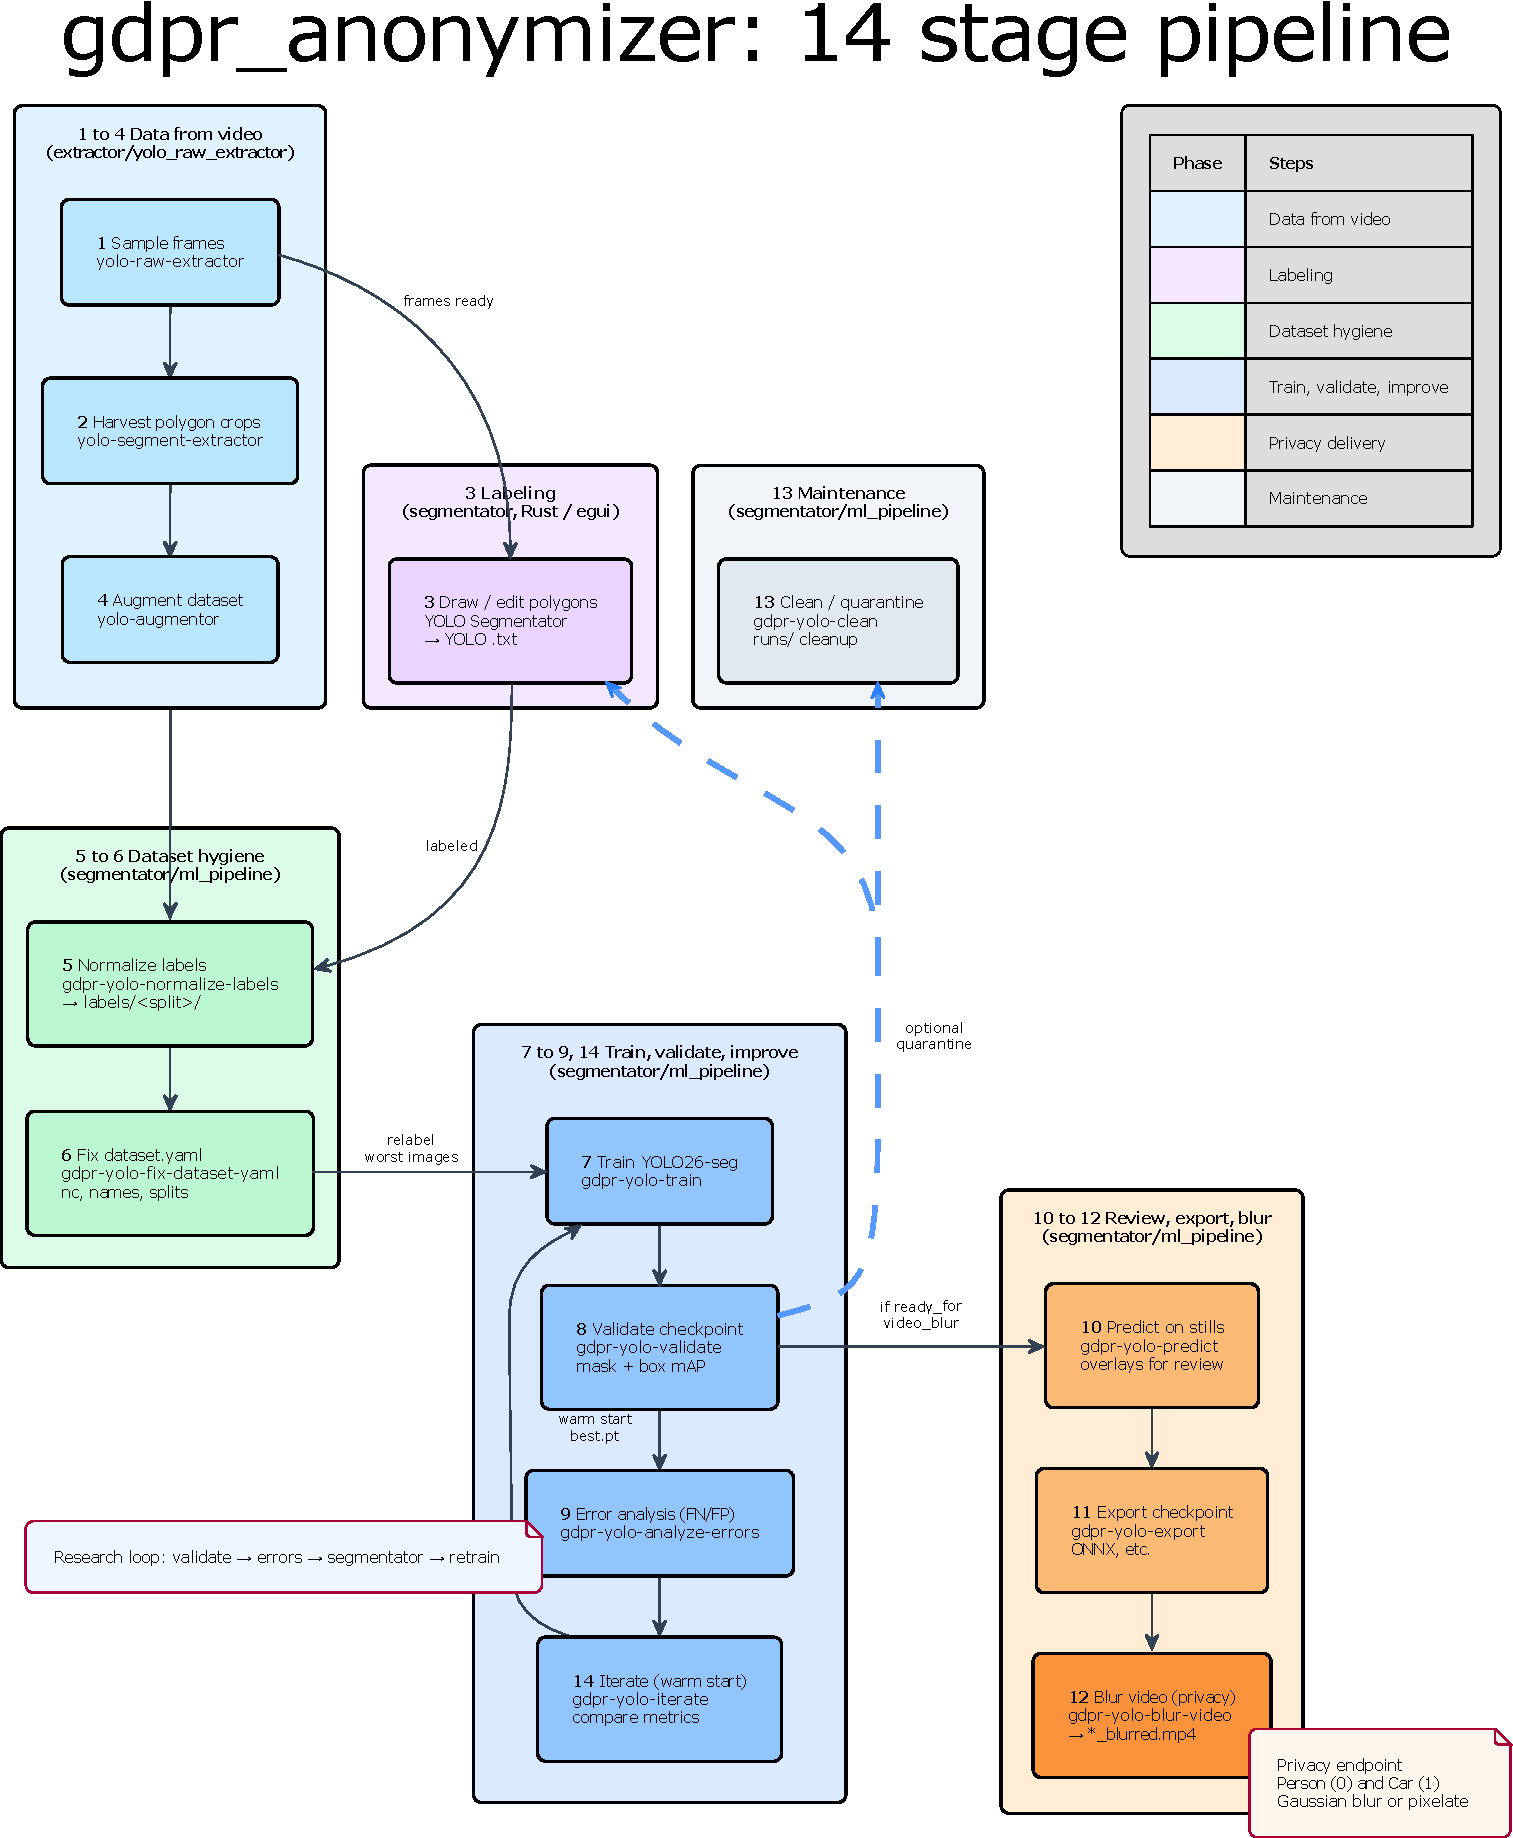
\includegraphics[width=0.88\textwidth]{images/pipeline14steps.pdf}
  \caption{Fourteen-stage privacy pipeline for the \texttt{gdpr\_anonymizer} project. Stages~1--4 correspond to the Python extractor package; stage~3 uses the Rust segmentator; stages~5--14 are provided by \texttt{segmentator/ml\_pipeline}.}
  \label{fig:pipeline14steps}
\end{figure}

Figure~\ref{fig:pipeline14steps} summarises the fourteen ordered stages from raw video to anonymised output. Steps~1--4 prepare data: frames are extracted, polygons are drawn in the desktop segmentator, segment crops are harvested for augmentation after labelling, and an augmented dataset copy is built. Steps~5--6 audit label layout and \texttt{dataset.yaml}. Steps~7--11 cover training, validation, error analysis, still-image prediction, and checkpoint export. Steps~12--14 deliver video blur, dataset or run-folder cleaning, and warm-started training iteration with metric comparison.

\begin{figure}[htbp]
  \centering
  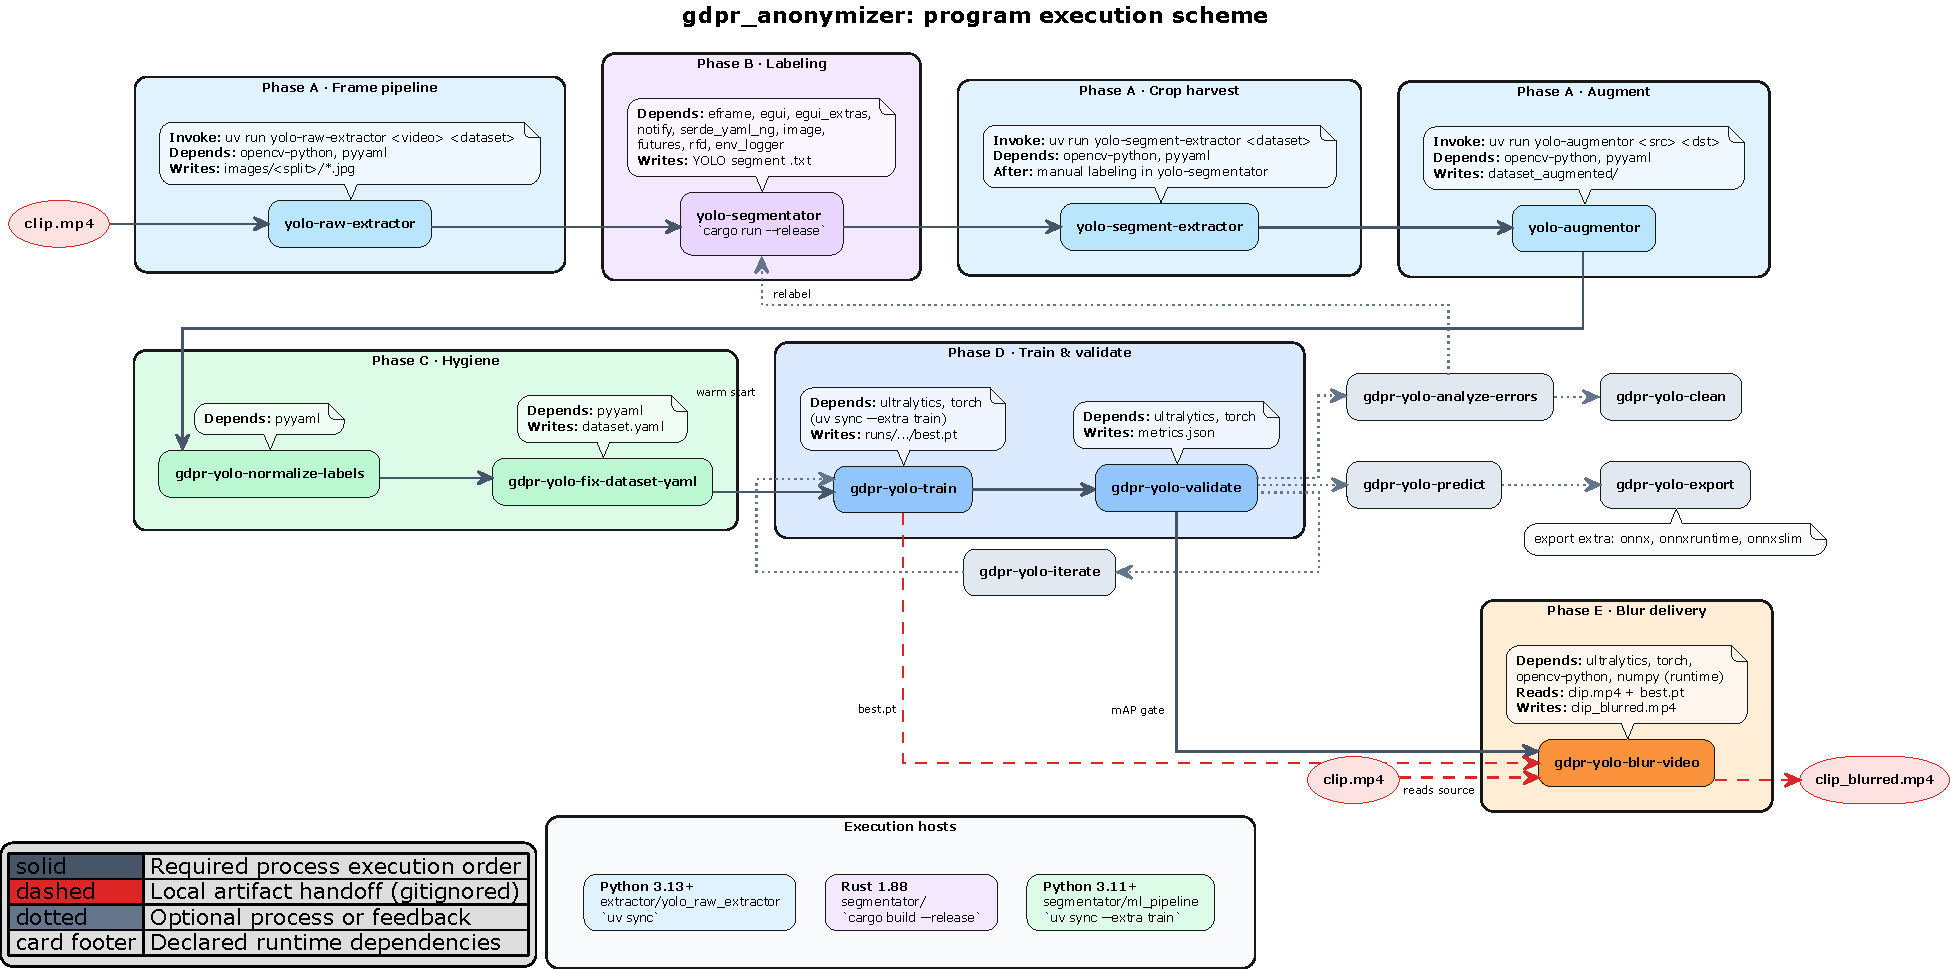
\includegraphics[width=\textwidth]{images/0_program_execution_scheme_manual.pdf}
  \caption{Program execution scheme for \texttt{gdpr\_anonymizer}. Solid arrows denote required process order; dashed arrows denote local artifact handoffs between stages; dotted arrows mark optional or feedback paths. Coloured phase bands group commands by package and runtime host (Python~3.13 extractor, Rust segmentator, Python~3.11 \texttt{ml\_pipeline}).}
  \label{fig:programexecscheme}
\end{figure}

Figure~\ref{fig:programexecscheme} maps the same workflow onto concrete CLI entry points and their runtime dependencies. Command names, flags, and worked examples are documented in the public repository README\footnote{\url{https://github.com/cguerreroto/gdpr_anonymizer/blob/main/README.md}}.

\section{Language and library choices}
\label{sec:languages}

The repository combines Rust and Python because annotation, machine-learning orchestration, and video I/O impose different constraints on responsiveness, dependency weight, and ecosystem access.

\subsection{Rust segmentator}

The desktop segmentator is implemented in Rust with \texttt{egui} and \texttt{eframe}. This stack was selected for a native polygon editor that watches dataset folders, refreshes image lists, and serialises YOLO segmentation labels beside each image with low UI latency. It corresponds to stage~3 in Figure~\ref{fig:pipeline14steps}. Dataset discovery, label parsing, and file watching are concentrated in \texttt{segmentator/src/dataset.rs}. Unit tests for label I/O live in inline \texttt{\#[cfg(test)]} modules next to the code they exercise.

\subsection{Python extractor and ML pipeline}

Two independent Python packages are managed with \texttt{uv}, each with its own \texttt{pyproject.toml} and lockfile. The extractor under \texttt{extractor/yolo\_raw\_extractor} targets Python~3.13 and handles frame extraction, segment cropping, and dataset augmentation (stages~1, 2, and~4 in Figure~\ref{fig:pipeline14steps}). The ML pipeline under \texttt{segmentator/ml\_pipeline} targets Python~3.11 for compatibility with Ultralytics and PyTorch and implements stages~5--14 of the same figure.

Training, validation, prediction, export, and video blur depend on the optional \texttt{[train]} extra (Ultralytics YOLO26-seg). ONNX export additionally requires the \texttt{[export]} extra. Layout and YAML utilities install after a plain \texttt{uv sync} without those extras, which keeps continuous integration lightweight. Video anonymisation reads and writes frames through OpenCV in \texttt{video.py}. Dataset hygiene, cleaning, iteration wrappers, and metric interpretation remain in standard-library-oriented modules with small, testable CLI entry points.

\subsection{Rationale for a hybrid layout}

Interactive labelling benefits from a compiled desktop application, whereas model training and batch CLIs benefit from the Python machine-learning ecosystem. The design replaces monolithic notebooks with path-based commands that can be composed in shell scripts or documented pipelines, which aligns with the staged layout shown in Figure~\ref{fig:pipeline14steps} and with reproducibility goals emphasised in the course material on clean code and pipelining.

\section{Project workflow setup}
\label{sec:workflow}

\subsection{Version control and pull requests}

The repository follows GitHub Flow: short-lived branches are created from \texttt{main}, changes are committed in focused units, and integration occurs through pull requests that reference issues where applicable \cite{GitHubFlow}. The contribution guide documents issue templates for bugs and feature requests, a pull-request checklist, and the expectation that \texttt{make test} passes before review \cite{ContributingGDPR}.

During early refactoring, some changes landed directly on \texttt{main} before branch protection and formal review were in place. Later work adopts the documented PR workflow. A maintainer checklist for branch protection and required status checks is kept locally and mirrors the settings described in the contribution guide.

\subsection{Continuous integration}

GitHub Actions workflow \texttt{ci.yml} runs on push and pull request to \texttt{main} \cite{CIGDPR}. Python jobs use a matrix over both packages (\texttt{extractor/yolo\_raw\_extractor} and \texttt{segmentator/ml\_pipeline}) on Ubuntu with \texttt{uv sync --group dev} followed by \texttt{pytest --cov}. Rust jobs install Linux GUI dependencies, then run \texttt{cargo test} and \texttt{cargo clippy -- -D warnings} in \texttt{segmentator}. Coverage XML artifacts are uploaded but no minimum percentage gate is enforced.

The root \texttt{Makefile} exposes the same commands for local verification: \texttt{make test}, \texttt{make lint}, \texttt{make fmt}, and \texttt{make coverage}. This duplication keeps developer commands aligned with CI without requiring contributors to memorise per-package paths.

\subsection{Repository presentation}

The public GitHub repository serves as the project face: a structured README, PolyForm Noncommercial License~1.0.0 \cite{PolyFormNC}, \texttt{AUTHORS.md}, dependency lockfiles, and \texttt{.gitignore} rules that exclude datasets, weights, and local documentation. Large binaries and sensitive paths are never committed; callers supply dataset and run directories on the command line.

\section{Project development setup}
\label{sec:devsetup}

\subsection{Virtual environments and dependencies}

Each Python package is installed in isolation with \texttt{uv sync} from its directory \cite{AstralUV}. Development tools (\texttt{pytest}, \texttt{pytest-cov}, \texttt{py-spy}) are pulled in via \texttt{--group dev}. Machine-learning commands require \texttt{uv sync --extra train}; ONNX export adds \texttt{--extra export}. Lockfiles are committed so reproducible installs are available on Linux CI runners and on local macOS workstations. A platform setup script under gitignored \texttt{local/} automates Rust, \texttt{uv}, and initial test execution for macOS contributors.

The Rust segmentator is built with \texttt{cargo build --release}. The pinned toolchain version is declared in \texttt{segmentator/Cargo.toml}.

\subsection{Integrated development environment}

Day-to-day editing is performed in a Visual Studio Code-compatible editor with the Rust Analyzer extension for the segmentator crate and the Python extension for both \texttt{uv} projects. Integrated terminals run \texttt{uv run} and \texttt{cargo} tasks from the repository root or from package subdirectories. This layout supports quick navigation between Rust UI code, Python CLIs, and their respective test suites.

\subsection{Linters, formatters, and profiling}

Rust sources are formatted with \texttt{cargo fmt} and checked with \texttt{cargo clippy -- -D warnings}, matching the CI job. Python modules follow the naming and typing conventions of surrounding code; no separate Python linter gate is configured in CI at present.

Optional profiling is documented in \texttt{PERFORMANCE.md}: Python \texttt{cProfile} and \texttt{py-spy} for extractor and pipeline stages, and \texttt{cargo flamegraph} for the segmentator when UI responsiveness must be investigated. Profiling remains a local concern and is not part of the default test workflow.

\section{Unit testing and coverage}
\label{sec:testing}

\subsection{Test layout}

Automated tests are organised in three suites documented in \texttt{tests/README.md} \cite{TestsGDPR}. The Rust segmentator exposes five unit tests in \texttt{dataset.rs} via \texttt{cargo test}. The extractor package contains 126 \texttt{pytest} cases under \texttt{extractor/yolo\_raw\_extractor/tests}. The ML pipeline package contains 291 \texttt{pytest} cases under \texttt{segmentator/ml\_pipeline/tests}. In total, 422 automated tests run from the repository root through \texttt{make test}.

Tests follow the arrange--act--assert pattern. Filesystem fixtures prefer \texttt{tmp\_path}. External stacks such as Ultralytics, OpenCV, and NumPy are not loaded in the default development or CI environment for \texttt{ml\_pipeline}; instead, factory injection, \texttt{pytest} \texttt{monkeypatch}, and shared fakes in \texttt{tests/fakes.py} exercise video blur, export, training, and validation code paths without downloading \texttt{.pt} weights or committing video fixtures \cite{UnittestMock,TestsGDPR}.

\subsection{\texttt{make test} versus \texttt{make coverage}}

These targets answer different questions. \texttt{make test} invokes \texttt{pytest} and \texttt{cargo test} without coverage instrumentation. The terminal output reports pass or fail counts and a compact per-file progress line for Python. It does not list line percentages.

\texttt{make coverage} runs \texttt{pytest --cov} in both Python packages with branch coverage enabled in each \texttt{pyproject.toml} \cite{PytestCov,CoveragePy}. The terminal report lists statement counts, missed lines, partial branches, and percentages per module, and writes HTML and XML reports under each package. CI Python jobs also pass \texttt{--cov} and upload \texttt{coverage.xml}, but they do not fail when coverage falls below a threshold. Rust coverage is optional through \texttt{cargo llvm-cov} and is excluded from \texttt{make coverage}.

\subsection{Coverage evolution in three phases}

Coverage was measured at three repository states by running the same \texttt{pytest --cov} commands after checking out each milestone. Cover1 marks the initial suite with \texttt{pytest-cov} wired (205 Python tests). Cover2 marks the expanded unit-test set immediately before systematic mocking of heavy imports (350 Python tests). Cover3 marks the current tree after mock-based tests closed remaining gaps (417 Python tests).

At Cover1, package totals were 82\% for \texttt{ml\_pipeline} and 41\% for the extractor. Modules that depend on OpenCV or Ultralytics, especially \texttt{video.py} at 55\%, remained largely untested because the dev install omits those dependencies. Cover2 raised totals to 90\% and 89\% through broader CLI and driver tests with stub factories, but \texttt{video.py} stayed at 60\% because real \texttt{cv2} and \texttt{numpy} imports were still avoided. Cover3 applied standard-library \texttt{unittest.mock} patterns together with \texttt{monkeypatch} to register lightweight fake modules before lazy imports run. Package totals reached 97\% while \texttt{video.py} rose to 95\% and \texttt{validate.py} to 99\%, without adding GPU hardware or binary fixtures to the repository.

Table~\ref{tab:coverage_summary} summarises package-level results. Module-level percentages for both Python packages are listed in Appendix~\ref{app:coverage_tables}. Rows with the largest Cover2 to Cover3 gains (\texttt{video.py}, \texttt{validate.py}, \texttt{cli\_dataset\_yaml.py}, \texttt{export.py}) correspond to code paths that were previously reachable only when optional ML stacks were installed.

\begin{table}[htbp]
\centering
\footnotesize
\begin{tabular}{@{}l r c c c c@{}}
\hline
\textbf{Phase} & \textbf{pytest cases} & \textbf{ml\_pipeline} & \textbf{extractor} & \textbf{video.py} & \textbf{validate.py} \\
\hline
Cover1 (initial suite) & 205 & 82\% & 41\% & 55\% & 87\% \\
Cover2 (pre-mocking) & 350 & 90\% & 89\% & 60\% & 87\% \\
Cover3 (after mocking) & 417 & 97\% & 97\% & 95\% & 99\% \\
\hline
\end{tabular}
\caption{Summary of Python test counts and coverage at three repository milestones. Rust segmentator tests (five cases) are excluded.}
\label{tab:coverage_summary}
\end{table}

The Rust segmentator suite is not included in \texttt{make coverage}. All suites pass under \texttt{make test} on the current tree.


\section{Conclusions and outlook}
\label{sec:conclusions}

This report described how \texttt{gdpr\_anonymizer} was designed, implemented, and verified as a local video-privacy toolchain. The following subsections summarise what the repository delivers today, how it behaves in practice, and which improvements remain open for future work.

\subsection{What was achieved}

The central outcome is a single public repository that accepts an MP4 file as input and produces a blurred MP4 as output, while keeping datasets, training runs, and model weights on the operator's machine and outside version control. The Python \texttt{extractor} and the Rust \texttt{segmentator} were present from the initial import of upstream tooling \cite{DecrypheExtractor,DecrypheSegmentator}; the contribution documented here is the \texttt{segmentator/ml\_pipeline} package, which closes the gap between hand-labelled polygons and an repeatable anonymisation endpoint through fourteen documented command-line stages \cite{RepoGDPR}.

At project start, the imported stack offered frame extraction, augmentation, and polygon labelling, but no in-repository training drivers, validation metrics, JSON reporting, unit-test harness, or video blur CLI. The work reported in Sections~\ref{sec:languages}--\ref{sec:testing} added dataset normalisation, portable \texttt{dataset.yaml} repair, YOLO26-seg training and validation, error analysis, optional export, explicit video blur, cleaning utilities, and warm-started iteration. Every pipeline command can emit structured JSON, which allows an operator to inspect counts, thresholds, and recommendations before deciding whether to label again, train again, or proceed to blur.

From a product perspective, the repository targets a practical privacy problem emphasised in the course presentation: sharing audiovisual material without consent exposes identifiable persons and, in many driving or street scenes, vehicle registration regions that must be obscured before publication. Regulation such as the GDPR \cite{GDPR2016} does not prescribe a specific technical method, but it reinforces that personal data should be processed lawfully and with appropriate safeguards. A documented open toolchain lowers the barrier for researchers who need reproducible control rather than ad hoc manual redaction.

To the author's knowledge, \texttt{gdpr\_anonymizer} is one of the few openly published pipelines that covers the full path from raw video through segmentation training to mask-based blur for both persons and cars in one repository. Many capable commercial products exist, yet they are often costly, closed, or limited to a single stage such as detection-only redaction or external training. The present design deliberately prioritises simplicity, explicit paths on the command line, and GitHub-hosted documentation so that others can audit, extend, or fork the workflow under the PolyForm Noncommercial licence \cite{PolyFormNC}.

Two qualitative properties distinguish the anonymisation approach from bounding-box-only redaction, as argued in the presentation material. First, instance \emph{segmentation} masks follow object contours; Gaussian or pixelated blur inside the mask union avoids the large rectangular boxes that leak background context around profile faces or partial vehicles and look conspicuous in social-media footage. Second, usable blur does not necessarily require a massive proprietary dataset at the outset. Experiments on short source clips already produced fairly convincing anonymisation when only a modest number of labelled frames were available; as more diverse footage containing pedestrians and cars is annotated, the same pipeline can yield a stronger pretrained checkpoint suitable for batch processing of new videos without redesigning the workflow.

\subsection{Does it work}

Empirical use confirms that the pipeline performs substantially better than initially expected for a student product scope. With relatively little labelled material extracted from short input videos, validation already reached bands where the interpretation layer marks \texttt{ready\_for\_video\_blur} in \texttt{metrics.json}, and the blur stage produced visually acceptable output on multi-thousand-frame clips. Reported blur KPIs include frame counts, detection rates, per-class totals, and average masked area fraction in \texttt{runs/blur/report.json}, which makes downstream review straightforward.

Quality still scales with data and labelling effort, as in any supervised segmentation project. More annotated frames, broader scene diversity, and careful polygon boundaries improve mask mAP and reduce missed or imprecise regions. The repository supports that growth without forcing the operator to restart from scratch: \texttt{gdpr-yolo-iterate} warm-starts a new training run from an existing \texttt{best.pt}, re-validates on the same split, and records metric deltas against a prior validation report. Combined with \texttt{gdpr-yolo-analyze-errors}, which surfaces worst validation images, the workflow implements a feedback loop from metrics back to labelling and training rather than a one-shot train-and-hope procedure.

Deployment remains local by design. Training and blur require the optional Ultralytics and PyTorch stack, yet neither a dedicated cloud service nor high-end GPU hardware is mandatory. CPU execution is supported throughout; a GPU mainly reduces wall-clock time on long videos or large epoch counts. Continuous integration on GitHub Actions runs the Rust and Python unit suites on every pull request \cite{CIGDPR}, and the coverage evolution summarised in Section~\ref{sec:testing} indicates that regressions in CLI drivers and video logic are unlikely to pass unnoticed.

\subsection{What remains to be done}

Several limitations are understood and documented rather than hidden. The most visible artefact in plate and small-object blur is temporal \emph{flickering}: when segmentation masks shift abruptly between neighbouring frames, the obscured region appears to jump even though each frame is processed correctly in isolation. A practical mitigation---not yet implemented---is temporal propagation of stable polygon or mask geometry. If frame~3 and frames~7--9 share substantially the same segment coordinates for a given instance, intermediate frames can inherit interpolated or held positions so that blur boundaries remain consistent across the clip. This is compatible with the existing per-frame blur architecture and would not require abandoning the current JSON-first CLI design.

Further gains depend primarily on dataset curation, which remains the responsibility of each operator. Better masks require more accurate polygons, especially on profile faces, partially occluded plates, and varied lighting. Presentation notes highlighted additional data axes: more pedestrian diversity, more licence-plate examples, plates from different countries, and enough epochs to stabilise small moving regions. Those are process recommendations rather than missing code paths; the augmentor, segmentator, and iteration tools already support incremental dataset growth.

Tooling inside the segmentator could also reduce labelling friction. A ``magic wand'' or assisted edge selection around faces and plate borders would accelerate polygon creation and improve boundary accuracy compared with purely manual vertex placement. Keyboard shortcuts, zoom, and scroll-bar improvements were already added to the Rust UI during the project; assisted selection would be a natural next ergonomic step.

Finally, integrating external detection datasets that ship bounding boxes but not segmentation polygons would require a conversion stage, as noted when evaluating public Roboflow face-detection corpora during the presentation. Such a step would sit beside the existing fourteen-stage table rather than replace mask-based training, because box-only labels cannot reproduce the contour-following blur that motivates the segmentation model choice.

In summary, \texttt{gdpr\_anonymizer} delivers a coherent, test-covered, locally runnable path from video ingest to GDPR-oriented anonymisation output. It already demonstrates that modest labelled data can produce useful blur, that segmentation masks outperform coarse boxes for visual quality, and that iteration hooks prevent dead-end training cycles. Remaining work centres on temporal stability in video blur, richer labelled data, and faster annotation assistance---extensions that build on the foundation described in this report rather than replacing it.


\newpage
% - - - - - - - - - - - -  - - - - - - - - - - - - - - - - - - - - - - - - %
%	References
% - - - - - - - - - - - -  - - - - - - - - - - - - - - - - - - - - - - - - %
% Local PDF copies may live in PDFs/ next to the main .tex file; filenames can match
% cite keys: Wang2004.pdf, Brunet2012.pdf, Channappayya2008.pdf, Brunet2017Handbook.pdf.

\begin{thebibliography}{99}

%    \bibitem{Wang2004}
%    {\sc Wang, Z., Bovik, A.~C., Sheikh, H.~R., and Simoncelli, E.~P.}
%    (2004).
%    Image quality assessment: from error visibility to structural similarity.
%    \textit{IEEE Transactions on Image Processing}, 13(4), 600--612.
%    
%    \bibitem{Brunet2012}
%    {\sc Brunet, D., Vrscay, E.~R., and Wang, Z.}
%    (2012).
%    On the mathematical properties of the structural similarity index.
%    \textit{IEEE Transactions on Image Processing}, 21(4), 1488--1499.
%    
%    \bibitem{Channappayya2008}
%    {\sc Channappayya, S.~S., Bovik, A.~C., Caramanis, C., and Heath, R.~W.}
%    (2008).
%    Design of linear equalizers optimized for the structural similarity index.
%    \textit{IEEE Transactions on Image Processing}, 17(6), 857--872.
%    
%    \bibitem{Brunet2017Handbook}
%    {\sc Brunet, D., Channappayya, S.~S., Wang, Z., Vrscay, E.~R., and Bovik, A.~C.}
%    (2017).
%    Optimizing image quality.
%    In {\sc Monga, V.} (ed.), \textit{Handbook of Convex Optimization Methods in Imaging Science}, pp.~15--41.
%    Springer, Cham.
%    \href{https://doi.org/10.1007/978-3-319-61609-4_2}{doi:10.1007/978-3-319-61609-4\_2}.
    
    \end{thebibliography}

\appendix
% - - - - - - - - - - - -  - - - - - - - - - - - - - - - - - - - - - - - - %
%	Appendices (order matches first citation in the main text: Results, then Discussion)
% - - - - - - - - - - - -  - - - - - - - - - - - - - - - - - - - - - - - - %
\newcommand{\appendixcaptionsuffix}{%
  \emph{Abbreviations:} AE: autoencoder; GA: genetic algorithm; PSO: particle swarm optimisation; MSE: mean squared error; Mem: memory usage; PSNR: peak signal-to-noise ratio; SSIM: structural similarity index measure; Time: wall-clock runtime.}

\section{Numerical results (tables)}
\label{sec:results_tables}

\begin{table}[H]
\centering
\footnotesize
\begin{tabular}{llcccccc}
\hline
Method & Mode & SSIM$_{c}$ $\uparrow$ & SSIM$_{n}$ $\uparrow$ & PSNR $\uparrow$ & MSE $\downarrow$ & Time $\downarrow$ & Mem $\downarrow$ \\
\hline
AE  & Blind  & 0.350 $\pm$ 0.001 & 0.965 $\pm$ 0.001 & 22.4 $\pm$ 0.1 & 0.0057 $\pm$ 0.0001 & 292.8 $\pm$ 2.1 & 1234 $\pm$ 7 \\
AE  & Hybrid & \textbf{0.809 $\pm$ 0.008} & 0.908 $\pm$ 0.005 & \textbf{28.8 $\pm$ 0.2} & \textbf{0.0013 $\pm$ 0.0001} & 298.8 $\pm$ 23.3 & 1239 $\pm$ 12 \\
GA  & Blind  & 0.241 $\pm$ 0.001 & \textbf{0.999 $\pm$ 0.000} & 17.0 $\pm$ 0.0 & 0.0199 $\pm$ 0.0000 & 83.3 $\pm$ 1.4 & 616 $\pm$ 17 \\
GA  & Hybrid & 0.257 $\pm$ 0.005 & \textbf{0.999 $\pm$ 0.000} & 17.8 $\pm$ 0.1 & 0.0167 $\pm$ 0.0003 & \textbf{70.6 $\pm$ 1.3} & 609 $\pm$ 2 \\
PSO & Blind  & 0.318 $\pm$ 0.039 & 0.988 $\pm$ 0.006 & 20.6 $\pm$ 0.8 & 0.0086 $\pm$ 0.0015 & 139.6 $\pm$ 56.9 & \textbf{545 $\pm$ 22} \\
PSO & Hybrid & 0.340 $\pm$ 0.013 & 0.986 $\pm$ 0.005 & 21.1 $\pm$ 0.4 & 0.0075 $\pm$ 0.0007 & 145.3 $\pm$ 50.5 & 563 $\pm$ 39 \\
\hline
\end{tabular}
\caption{Global comparison of the evaluated denoising methods. SSIM$_c$ denotes SSIM between the estimate and the clean image, while SSIM$_n$ denotes SSIM between the estimate and the noisy input. Results are reported as mean $\pm$ standard deviation.\protect\appendixcaptionsuffix}
\label{tab:global_results_compact}
\end{table}

\begin{table}[H]
\centering
\footnotesize
\begin{tabular}{llcccccc}
\hline
Method & Mode & SSIM$_{c}$ $\uparrow$ & SSIM$_{n}$ $\uparrow$ & PSNR $\uparrow$ & MSE $\downarrow$ & Time $\downarrow$ & Mem $\downarrow$ \\
\hline
GA  & Blind  & 0.241 $\pm$ 0.001 & 0.999 $\pm$ 0.000 & 17.0 $\pm$ 0.0 & 0.0199 $\pm$ 0.0000 & 251.5 $\pm$ 0.0 & 228 $\pm$ 0 \\
GA  & Hybrid & 0.260 $\pm$ 0.002 & 0.999 $\pm$ 0.000 & 17.9 $\pm$ 0.1 & 0.0164 $\pm$ 0.0001 & 247.8 $\pm$ 1.2 & 229 $\pm$ 1 \\
PSO & Blind  & 0.373 $\pm$ 0.006 & 0.988 $\pm$ 0.001 & 21.9 $\pm$ 0.1 & 0.0064 $\pm$ 0.0001 & 436.2 $\pm$ 12.1 & 210 $\pm$ 3 \\
PSO & Hybrid & \textbf{0.533 $\pm$ 0.007} & 0.963 $\pm$ 0.003 & \textbf{25.1 $\pm$ 0.1} & \textbf{0.0031 $\pm$ 0.0001} & 430.5 $\pm$ 14.7 & \textbf{205 $\pm$ 2} \\
\hline
\end{tabular}
\caption{Patchwise comparison of GA and PSO methods. SSIM$_c$ denotes SSIM between the estimate and the clean image, while SSIM$_n$ denotes SSIM between the estimate and the noisy input. Results are reported as mean $\pm$ standard deviation.\protect\appendixcaptionsuffix}
\label{tab:patchwise_results}
\end{table}


\section{Runtime overview (bar chart)}
\label{sec:runtime_bars}

\begin{figure}[H]
  \centering
  \includegraphics[width=\textwidth]{images/runtime_bars.png}
  \caption{Mean wall-clock runtime by method and mode (global \emph{vs.\ }patchwise where applicable). The chart mirrors the Time column in Tables~\ref{tab:global_results_compact} and~\ref{tab:patchwise_results} and highlights relative computational cost at a glance. The autoencoder appears in global mode only: a patchwise AE would require training a separate model per patch, which conflicts with the usual end-to-end convolutional autoencoder objective and would imply prohibitive aggregate training time, so we omit that bar. GA and PSO remain reported in both geometries because patchwise search does not entail retraining a network for each tile.\protect\appendixcaptionsuffix}
  \label{fig:runtime_bars}
\end{figure}


\section{Denoised images: visual comparisons}
\label{sec:denoised_images}

\begin{figure}[H]
  \centering
  \includegraphics[width=\textwidth]{images/B_u_v_best_AE_GA_PSO_final.png}
  \caption{Best denoised output per method. From left to right: clean reference $u$, noisy input $v$, AE hybrid (1000 epochs, $\mathrm{SSIM}_c = 0.809$), GA hybrid patchwise ($\mathrm{SSIM}_c = 0.260$), PSO hybrid patchwise ($\mathrm{SSIM}_c = 0.533$).\protect\appendixcaptionsuffix}
  \label{fig:best_denoised}
\end{figure}

\begin{figure}[H]
  \centering
  \includegraphics[width=1\textwidth]{images/B_composite_ga_global_vs_patchwise.png}
  \caption{GA search approach compared in hybrid mode. From left to right: clean reference $u$, noisy input $v$, GA global ($\mathrm{SSIM}_c = 0.257$), GA patchwise ($\mathrm{SSIM}_c = 0.260$). While the metric gain is negligible, a subtle visual improvement is nonetheless perceptible.\protect\appendixcaptionsuffix}
  \label{fig:ga_global_patchwise}
\end{figure}

\begin{figure}[H]
  \centering
  \includegraphics[width=1\textwidth]{images/B_composite_pso_global_vs_patchwise.png}
  \caption{PSO search approach compared in hybrid mode. From left to right: clean reference $u$, noisy input $v$, PSO global ($\mathrm{SSIM}_c = 0.340$), PSO patchwise ($\mathrm{SSIM}_c = 0.533$). The patchwise decomposition yields a substantial improvement in both metrics and visual quality.\protect\appendixcaptionsuffix}
  \label{fig:pso_global_patchwise}
\end{figure}

\begin{figure}[H]
  \centering
  \includegraphics[width=1\textwidth]{images/B_composite_ae_blind_vs_hybrid.png}
  \caption{Autoencoder denoising modes compared. From left to right: clean reference $u$, noisy input $v$, AE blind ($\mathrm{SSIM}_c = 0.350$), AE hybrid ($\mathrm{SSIM}_c = 0.809$). All outputs correspond to seed s11, 1000 epochs.\protect\appendixcaptionsuffix}
  \label{fig:ae_blind_hybrid}
\end{figure}

\begin{figure}[H]
  \centering
  \includegraphics[width=1\textwidth]{images/B_composite_ae_e1000_hybrid_seed_consistency.png}
  \caption{Seed consistency of the AE in hybrid mode (1000 epochs). From left to right: clean reference $u$, noisy input $v$, seed s11, seed s22, seed s33. The near-identical outputs confirm low stochastic variability ($\mathrm{SSIM}_c = 0.809 \pm 0.008$).\protect\appendixcaptionsuffix}
  \label{fig:ae_seeds}
\end{figure}


\section{Quality \emph{vs.\ }runtime scatter plots}
\label{sec:plots}

\begin{figure}[H]
    \centering
    \begin{subfigure}[b]{0.45\textwidth}
        \includegraphics[width=\textwidth]{images/A_quality_vs_runtime_blind.png}
        \caption*{(a)}
    \end{subfigure}
    \hfill
    \begin{subfigure}[b]{0.45\textwidth}
        \includegraphics[width=\textwidth]{images/A_quality_vs_runtime_hybrid.png}
        \caption*{(b)}
    \end{subfigure}
    \caption{\textbf{Quality \emph{vs.\ }runtime scatter plots.} Runtime \emph{vs.\ }reconstruction quality under blind loss~(a) and hybrid loss~(b). Each point represents one run (seed); colour encodes the method (blue: AE, green: GA, orange: PSO), and marker fill encodes the search geometry (filled: global, outline: patchwise). The dashed vertical line marks the noisy baseline $\mathrm{SSIM}(v, u) = 0.350$. Under blind loss, all methods cluster near the baseline, consistent with the trivial solution $\hat{u} \approx v$. Under hybrid loss, the autoencoder achieves substantially higher quality, while PSO patchwise reaches $\mathrm{SSIM}_c = 0.533$ and GA remains near the baseline regardless of search geometry.\protect\appendixcaptionsuffix}
    \label{fig:loss_plots}
\end{figure}

\newpage
\section{Classical full-reference metrics (MSE and PSNR)}
\label{app:mse_psnr}

This appendix records standard pixelwise measures used only for benchmarking when a ground-truth image $u$ and an estimate $\hat{u}$ are both available. They are not terms in the optimisation objective $\mathcal{L}$ of Section~\ref{sec:loss_constraints}.

For vectorised images of length $n$ with dynamic range $[0,L]$ (e.g.\ $L=1$ after normalisation or $L=255$ for 8-bit storage), the mean squared error is
\begin{equation}
\label{eq:app_mse}
\mathrm{MSE}(u,\hat{u}) = \frac{1}{n}\sum_{k=1}^{n}(u_k-\hat{u}_k)^2.
\end{equation}
The peak signal-to-noise ratio in decibels is
\begin{equation}
\label{eq:app_psnr}
\mathrm{PSNR}(u,\hat{u}) = 10\log_{10}\!\left(\frac{L^2}{\mathrm{MSE}(u,\hat{u})}\right),
\end{equation}
with the convention $\mathrm{PSNR}=+\infty$ if $\mathrm{MSE}=0$. PSNR is a monotone function of MSE for fixed $L$; reporting both on the same pair $(u,\hat{u})$ is redundant unless raw MSE is needed for statistical analysis.

For comparison with the SSIM-based objective, full-reference SSIM$(\hat{u},u)$ (pooled over patches as in \eqref{eq:ssim_global_mean}) is the primary perceptual score; PSNR remains useful as a classical baseline cited alongside prior work.


%%% - - - - - - - - - - - -  - - - - - - - - - - - - - - - - - - - - - - - - %
%	References
% - - - - - - - - - - - -  - - - - - - - - - - - - - - - - - - - - - - - - %
% Local PDF copies may live in PDFs/ next to the main .tex file; filenames can match
% cite keys: Wang2004.pdf, Brunet2012.pdf, Channappayya2008.pdf, Brunet2017Handbook.pdf.

\begin{thebibliography}{99}

%    \bibitem{Wang2004}
%    {\sc Wang, Z., Bovik, A.~C., Sheikh, H.~R., and Simoncelli, E.~P.}
%    (2004).
%    Image quality assessment: from error visibility to structural similarity.
%    \textit{IEEE Transactions on Image Processing}, 13(4), 600--612.
%    
%    \bibitem{Brunet2012}
%    {\sc Brunet, D., Vrscay, E.~R., and Wang, Z.}
%    (2012).
%    On the mathematical properties of the structural similarity index.
%    \textit{IEEE Transactions on Image Processing}, 21(4), 1488--1499.
%    
%    \bibitem{Channappayya2008}
%    {\sc Channappayya, S.~S., Bovik, A.~C., Caramanis, C., and Heath, R.~W.}
%    (2008).
%    Design of linear equalizers optimized for the structural similarity index.
%    \textit{IEEE Transactions on Image Processing}, 17(6), 857--872.
%    
%    \bibitem{Brunet2017Handbook}
%    {\sc Brunet, D., Channappayya, S.~S., Wang, Z., Vrscay, E.~R., and Bovik, A.~C.}
%    (2017).
%    Optimizing image quality.
%    In {\sc Monga, V.} (ed.), \textit{Handbook of Convex Optimization Methods in Imaging Science}, pp.~15--41.
%    Springer, Cham.
%    \href{https://doi.org/10.1007/978-3-319-61609-4_2}{doi:10.1007/978-3-319-61609-4\_2}.
    
    \end{thebibliography} 


%%\input{sections/3_discussion.tex}
%%\newpage
%%
%%{
%%\color{red} \Huge \section*{\colorbox{yellow}{{ USE THIS INFO in color FOR THE PRESENTATION}}}
%%\vspace{-1em}
%%\color{red} \Huge \section*{\colorbox{yellow}{{ OR YOUR IMPLEMENTATION }}}
%%\vspace{-1em}
%%}
%%{\color{blue}\input{sections/2_ae.tex}}
%%\newpage
%%{\color{cyan}\input{sections/2_ga.tex}}
%%\newpage
%%{\color{magenta}\input{sections/2_pso.tex}}
%%
%%\appendix
%%% - - - - - - - - - - - -  - - - - - - - - - - - - - - - - - - - - - - - - %
%	Appendices (order matches first citation in the main text: Results, then Discussion)
% - - - - - - - - - - - -  - - - - - - - - - - - - - - - - - - - - - - - - %
\newcommand{\appendixcaptionsuffix}{%
  \emph{Abbreviations:} AE: autoencoder; GA: genetic algorithm; PSO: particle swarm optimisation; MSE: mean squared error; Mem: memory usage; PSNR: peak signal-to-noise ratio; SSIM: structural similarity index measure; Time: wall-clock runtime.}

\section{Numerical results (tables)}
\label{sec:results_tables}

\begin{table}[H]
\centering
\footnotesize
\begin{tabular}{llcccccc}
\hline
Method & Mode & SSIM$_{c}$ $\uparrow$ & SSIM$_{n}$ $\uparrow$ & PSNR $\uparrow$ & MSE $\downarrow$ & Time $\downarrow$ & Mem $\downarrow$ \\
\hline
AE  & Blind  & 0.350 $\pm$ 0.001 & 0.965 $\pm$ 0.001 & 22.4 $\pm$ 0.1 & 0.0057 $\pm$ 0.0001 & 292.8 $\pm$ 2.1 & 1234 $\pm$ 7 \\
AE  & Hybrid & \textbf{0.809 $\pm$ 0.008} & 0.908 $\pm$ 0.005 & \textbf{28.8 $\pm$ 0.2} & \textbf{0.0013 $\pm$ 0.0001} & 298.8 $\pm$ 23.3 & 1239 $\pm$ 12 \\
GA  & Blind  & 0.241 $\pm$ 0.001 & \textbf{0.999 $\pm$ 0.000} & 17.0 $\pm$ 0.0 & 0.0199 $\pm$ 0.0000 & 83.3 $\pm$ 1.4 & 616 $\pm$ 17 \\
GA  & Hybrid & 0.257 $\pm$ 0.005 & \textbf{0.999 $\pm$ 0.000} & 17.8 $\pm$ 0.1 & 0.0167 $\pm$ 0.0003 & \textbf{70.6 $\pm$ 1.3} & 609 $\pm$ 2 \\
PSO & Blind  & 0.318 $\pm$ 0.039 & 0.988 $\pm$ 0.006 & 20.6 $\pm$ 0.8 & 0.0086 $\pm$ 0.0015 & 139.6 $\pm$ 56.9 & \textbf{545 $\pm$ 22} \\
PSO & Hybrid & 0.340 $\pm$ 0.013 & 0.986 $\pm$ 0.005 & 21.1 $\pm$ 0.4 & 0.0075 $\pm$ 0.0007 & 145.3 $\pm$ 50.5 & 563 $\pm$ 39 \\
\hline
\end{tabular}
\caption{Global comparison of the evaluated denoising methods. SSIM$_c$ denotes SSIM between the estimate and the clean image, while SSIM$_n$ denotes SSIM between the estimate and the noisy input. Results are reported as mean $\pm$ standard deviation.\protect\appendixcaptionsuffix}
\label{tab:global_results_compact}
\end{table}

\begin{table}[H]
\centering
\footnotesize
\begin{tabular}{llcccccc}
\hline
Method & Mode & SSIM$_{c}$ $\uparrow$ & SSIM$_{n}$ $\uparrow$ & PSNR $\uparrow$ & MSE $\downarrow$ & Time $\downarrow$ & Mem $\downarrow$ \\
\hline
GA  & Blind  & 0.241 $\pm$ 0.001 & 0.999 $\pm$ 0.000 & 17.0 $\pm$ 0.0 & 0.0199 $\pm$ 0.0000 & 251.5 $\pm$ 0.0 & 228 $\pm$ 0 \\
GA  & Hybrid & 0.260 $\pm$ 0.002 & 0.999 $\pm$ 0.000 & 17.9 $\pm$ 0.1 & 0.0164 $\pm$ 0.0001 & 247.8 $\pm$ 1.2 & 229 $\pm$ 1 \\
PSO & Blind  & 0.373 $\pm$ 0.006 & 0.988 $\pm$ 0.001 & 21.9 $\pm$ 0.1 & 0.0064 $\pm$ 0.0001 & 436.2 $\pm$ 12.1 & 210 $\pm$ 3 \\
PSO & Hybrid & \textbf{0.533 $\pm$ 0.007} & 0.963 $\pm$ 0.003 & \textbf{25.1 $\pm$ 0.1} & \textbf{0.0031 $\pm$ 0.0001} & 430.5 $\pm$ 14.7 & \textbf{205 $\pm$ 2} \\
\hline
\end{tabular}
\caption{Patchwise comparison of GA and PSO methods. SSIM$_c$ denotes SSIM between the estimate and the clean image, while SSIM$_n$ denotes SSIM between the estimate and the noisy input. Results are reported as mean $\pm$ standard deviation.\protect\appendixcaptionsuffix}
\label{tab:patchwise_results}
\end{table}


\section{Runtime overview (bar chart)}
\label{sec:runtime_bars}

\begin{figure}[H]
  \centering
  \includegraphics[width=\textwidth]{images/runtime_bars.png}
  \caption{Mean wall-clock runtime by method and mode (global \emph{vs.\ }patchwise where applicable). The chart mirrors the Time column in Tables~\ref{tab:global_results_compact} and~\ref{tab:patchwise_results} and highlights relative computational cost at a glance. The autoencoder appears in global mode only: a patchwise AE would require training a separate model per patch, which conflicts with the usual end-to-end convolutional autoencoder objective and would imply prohibitive aggregate training time, so we omit that bar. GA and PSO remain reported in both geometries because patchwise search does not entail retraining a network for each tile.\protect\appendixcaptionsuffix}
  \label{fig:runtime_bars}
\end{figure}


\section{Denoised images: visual comparisons}
\label{sec:denoised_images}

\begin{figure}[H]
  \centering
  \includegraphics[width=\textwidth]{images/B_u_v_best_AE_GA_PSO_final.png}
  \caption{Best denoised output per method. From left to right: clean reference $u$, noisy input $v$, AE hybrid (1000 epochs, $\mathrm{SSIM}_c = 0.809$), GA hybrid patchwise ($\mathrm{SSIM}_c = 0.260$), PSO hybrid patchwise ($\mathrm{SSIM}_c = 0.533$).\protect\appendixcaptionsuffix}
  \label{fig:best_denoised}
\end{figure}

\begin{figure}[H]
  \centering
  \includegraphics[width=1\textwidth]{images/B_composite_ga_global_vs_patchwise.png}
  \caption{GA search approach compared in hybrid mode. From left to right: clean reference $u$, noisy input $v$, GA global ($\mathrm{SSIM}_c = 0.257$), GA patchwise ($\mathrm{SSIM}_c = 0.260$). While the metric gain is negligible, a subtle visual improvement is nonetheless perceptible.\protect\appendixcaptionsuffix}
  \label{fig:ga_global_patchwise}
\end{figure}

\begin{figure}[H]
  \centering
  \includegraphics[width=1\textwidth]{images/B_composite_pso_global_vs_patchwise.png}
  \caption{PSO search approach compared in hybrid mode. From left to right: clean reference $u$, noisy input $v$, PSO global ($\mathrm{SSIM}_c = 0.340$), PSO patchwise ($\mathrm{SSIM}_c = 0.533$). The patchwise decomposition yields a substantial improvement in both metrics and visual quality.\protect\appendixcaptionsuffix}
  \label{fig:pso_global_patchwise}
\end{figure}

\begin{figure}[H]
  \centering
  \includegraphics[width=1\textwidth]{images/B_composite_ae_blind_vs_hybrid.png}
  \caption{Autoencoder denoising modes compared. From left to right: clean reference $u$, noisy input $v$, AE blind ($\mathrm{SSIM}_c = 0.350$), AE hybrid ($\mathrm{SSIM}_c = 0.809$). All outputs correspond to seed s11, 1000 epochs.\protect\appendixcaptionsuffix}
  \label{fig:ae_blind_hybrid}
\end{figure}

\begin{figure}[H]
  \centering
  \includegraphics[width=1\textwidth]{images/B_composite_ae_e1000_hybrid_seed_consistency.png}
  \caption{Seed consistency of the AE in hybrid mode (1000 epochs). From left to right: clean reference $u$, noisy input $v$, seed s11, seed s22, seed s33. The near-identical outputs confirm low stochastic variability ($\mathrm{SSIM}_c = 0.809 \pm 0.008$).\protect\appendixcaptionsuffix}
  \label{fig:ae_seeds}
\end{figure}


\section{Quality \emph{vs.\ }runtime scatter plots}
\label{sec:plots}

\begin{figure}[H]
    \centering
    \begin{subfigure}[b]{0.45\textwidth}
        \includegraphics[width=\textwidth]{images/A_quality_vs_runtime_blind.png}
        \caption*{(a)}
    \end{subfigure}
    \hfill
    \begin{subfigure}[b]{0.45\textwidth}
        \includegraphics[width=\textwidth]{images/A_quality_vs_runtime_hybrid.png}
        \caption*{(b)}
    \end{subfigure}
    \caption{\textbf{Quality \emph{vs.\ }runtime scatter plots.} Runtime \emph{vs.\ }reconstruction quality under blind loss~(a) and hybrid loss~(b). Each point represents one run (seed); colour encodes the method (blue: AE, green: GA, orange: PSO), and marker fill encodes the search geometry (filled: global, outline: patchwise). The dashed vertical line marks the noisy baseline $\mathrm{SSIM}(v, u) = 0.350$. Under blind loss, all methods cluster near the baseline, consistent with the trivial solution $\hat{u} \approx v$. Under hybrid loss, the autoencoder achieves substantially higher quality, while PSO patchwise reaches $\mathrm{SSIM}_c = 0.533$ and GA remains near the baseline regardless of search geometry.\protect\appendixcaptionsuffix}
    \label{fig:loss_plots}
\end{figure}

\newpage
\section{Classical full-reference metrics (MSE and PSNR)}
\label{app:mse_psnr}

This appendix records standard pixelwise measures used only for benchmarking when a ground-truth image $u$ and an estimate $\hat{u}$ are both available. They are not terms in the optimisation objective $\mathcal{L}$ of Section~\ref{sec:loss_constraints}.

For vectorised images of length $n$ with dynamic range $[0,L]$ (e.g.\ $L=1$ after normalisation or $L=255$ for 8-bit storage), the mean squared error is
\begin{equation}
\label{eq:app_mse}
\mathrm{MSE}(u,\hat{u}) = \frac{1}{n}\sum_{k=1}^{n}(u_k-\hat{u}_k)^2.
\end{equation}
The peak signal-to-noise ratio in decibels is
\begin{equation}
\label{eq:app_psnr}
\mathrm{PSNR}(u,\hat{u}) = 10\log_{10}\!\left(\frac{L^2}{\mathrm{MSE}(u,\hat{u})}\right),
\end{equation}
with the convention $\mathrm{PSNR}=+\infty$ if $\mathrm{MSE}=0$. PSNR is a monotone function of MSE for fixed $L$; reporting both on the same pair $(u,\hat{u})$ is redundant unless raw MSE is needed for statistical analysis.

For comparison with the SSIM-based objective, full-reference SSIM$(\hat{u},u)$ (pooled over patches as in \eqref{eq:ssim_global_mean}) is the primary perceptual score; PSNR remains useful as a classical baseline cited alongside prior work.

%%
%%% - - - - - - - - - - - -  - - - - - - - - - - - - - - - - - - - - - - - - %
%	References
% - - - - - - - - - - - -  - - - - - - - - - - - - - - - - - - - - - - - - %
% Local PDF copies may live in PDFs/ next to the main .tex file; filenames can match
% cite keys: Wang2004.pdf, Brunet2012.pdf, Channappayya2008.pdf, Brunet2017Handbook.pdf.

\begin{thebibliography}{99}

%    \bibitem{Wang2004}
%    {\sc Wang, Z., Bovik, A.~C., Sheikh, H.~R., and Simoncelli, E.~P.}
%    (2004).
%    Image quality assessment: from error visibility to structural similarity.
%    \textit{IEEE Transactions on Image Processing}, 13(4), 600--612.
%    
%    \bibitem{Brunet2012}
%    {\sc Brunet, D., Vrscay, E.~R., and Wang, Z.}
%    (2012).
%    On the mathematical properties of the structural similarity index.
%    \textit{IEEE Transactions on Image Processing}, 21(4), 1488--1499.
%    
%    \bibitem{Channappayya2008}
%    {\sc Channappayya, S.~S., Bovik, A.~C., Caramanis, C., and Heath, R.~W.}
%    (2008).
%    Design of linear equalizers optimized for the structural similarity index.
%    \textit{IEEE Transactions on Image Processing}, 17(6), 857--872.
%    
%    \bibitem{Brunet2017Handbook}
%    {\sc Brunet, D., Channappayya, S.~S., Wang, Z., Vrscay, E.~R., and Bovik, A.~C.}
%    (2017).
%    Optimizing image quality.
%    In {\sc Monga, V.} (ed.), \textit{Handbook of Convex Optimization Methods in Imaging Science}, pp.~15--41.
%    Springer, Cham.
%    \href{https://doi.org/10.1007/978-3-319-61609-4_2}{doi:10.1007/978-3-319-61609-4\_2}.
    
    \end{thebibliography} 






%\begin{figure}[h!]
%\centering
%\includegraphics[width=0.4\textwidth]{images/2_knn_flowchart}
%\caption{\textbf{KNN algorithm.} A flowchart explaining the $k$NN algorithm}
%\label{fig_knnalgorithm}
%\end{figure}


%Use accuracy for balanced datasets where both classes are equally important.
%Use precision, recall, and F1-score for imbalanced datasets or when specific error types are more critical.
%Use IoU or Dice coefficient in segmentation tasks to evaluate mask quality.
%Use AUC-ROC when thresholds and class separation matter.



% https://www.mercity.ai/blog-post/building-medical-ai-assistants-with-visual-llms
% MEDITRON https://github.com/epfLLM/meditron?tab=readme-ov-file

%%%%% THIS IS THE ARTICLE
% https://arxiv.org/pdf/2303.00915v2
% https://github.com/microsoft/BiomedCLIP_data_pipeline/blob/main/README.md
% https://huggingface.co/microsoft/BiomedCLIP-PubMedBERT_256-vit_base_patch16_224
% EXAMPLE: https://huggingface.co/microsoft/BiomedCLIP-PubMedBERT_256-vit_base_patch16_224/blob/main/biomed_clip_example.ipynb


% \includepdf[scale=0.90, nup=2x2, pages={1-4}, 
% 	pagecommand= \section{Assignment 1: pngq.c} \label{SP_assignment1_2023},
%	offset=-0.0in -0.50in 0.0in 0.0in,
%	delta=-0.25in -0.45in]{
%	pdfs/lorem.pdf
%	}

\end{document} 